\chapter{Idea rozwiązania i algorytmy}
\thispagestyle{chapterBeginStyle}
\label{rozdzial2}

Głównym celem pracy jest stworzenie prostego modelu sztucznej inteligencji do grania w warcaby w~wariancie angielskim z pewną strategią. Istnieją różne podejścia do tego zagadnienia, spośród których najpopularniejszymi są te stosujące sieci neuronowe (zestawem danych byłaby np. baza meczów rozegranych na mistrzostwach na przestrzeni kilkunastu lat). Praca skupia się na algorytmie Minimax połączonym z~funkcją oceny heurystycznej. Do częściowego wyznaczenia funkcji oceny wykorzystano odmianę algorytmu genetycznego.

\section{Minimax}

Minimax jest szczególną wersją algorytmu przeszukującego w grafie. Jego idea jest bardzo prosta i~zbliżona do ludzkiego rozumowania. Mając dany stan planszy oraz głębokość przeszukiwania, algorytm rekurencyjnie rozpatruje kolejne stany planszy symulując wykonanie jednego możliwego ruchu~(Rys.~\ref{fig:kolejnosc}). Kiedy już osiągnie maksymalną głębokość przeszukiwań na którymś stanie, funkcją oceny heurystycznej przypisuje wartość do tego stanu, po czym zwraca tę wartość do stanu-rodzica. Mając wartości oceny od każdego swojego dziecka, stan wybiera jedną z nich i przekazuje ją do swojego rodzica. Gdy wybór dojdzie do stanu będącego korzeniem drzewa przeszukiwań, algorytm wybierze jedną z dostępnych mu ocen i zwróci ruch do stanu, któremu ta ocena odpowiada.

{\small
\begin{pseudokod}[H]
%\SetAlTitleFnt{small}
\SetArgSty{normalfont}
\SetKwFunction{Evaluate}{evaluateState}
\SetKwFunction{Children}{getChildren}
\SetKwFunction{Minimax}{minimax}
\KwIn{Stan gry $state$, flaga gracza $perspective$, głębokość przeszukiwań $h$, rozpatrujący gracz $player$}
\KwOut{Wartość funkcji oceny $eval$}
\eIf{$h = 0$}{
$eval \leftarrow \Evaluate{state, player}$\;
}{
\eIf{$perspective = MAX$}{
$maxEval \leftarrow -\infty$\;
\ForEach{$child \in \Children{state}$}{
$childEval \leftarrow \Minimax{child, MIN, h - 1, player}$\;
\If{$childEval \ge maxEval$}{
$maxEval \leftarrow childEval$
% $bestState \leftarrow child$
}
}
% $state \leftarrow bestState$
$eval \leftarrow maxEval$
}{
$minEval \leftarrow +\infty$\;
\ForEach{$child \in \Children{state}$}{
$childEval \leftarrow \Minimax{child, MAX, h - 1, player}$\;
\If{$childEval \le minEval$}{
$minEval \leftarrow childEval$
% $bestState \leftarrow child$
}
}
% $state \leftarrow bestState$
$eval \leftarrow minEval$
}
}
\caption{Prosty algorytm Minimax}\label{alg:mine}
\end{pseudokod}
}

% TODO: new page, albo vspace
\vspace{1cm}

Swoją nazwę algorytm zawdzięcza naprzemiennemu rozpatrywaniu ocen heurystycznych w drzewie przeszukiwań. W momencie gdy dany gracz wywołuje procedurę Minimaxa rozpatrując możliwe do wykonania przez niego ruchy, oznaczany jest jako gracz MAX. W powstałych stanach gry gracz symuluje tok rozumowania jego przeciwnika, rozpatrując ruchy za niego i oznaczając go jako gracza MIN. Stany na kolejnym poziomie w drzewie przeszukiwań rozpatruje gracz MAX, i tak dalej. Gdy gracz MAX dokonuje wyboru oceny do przekazania do stanu-rodzica, wybiera maksymalną wartość. Analogicznie, gracz MIN wybiera ocenę o minimalnej wartości.~(Rys.~\ref{fig:minimax})

\begin{figure}
    \centering
    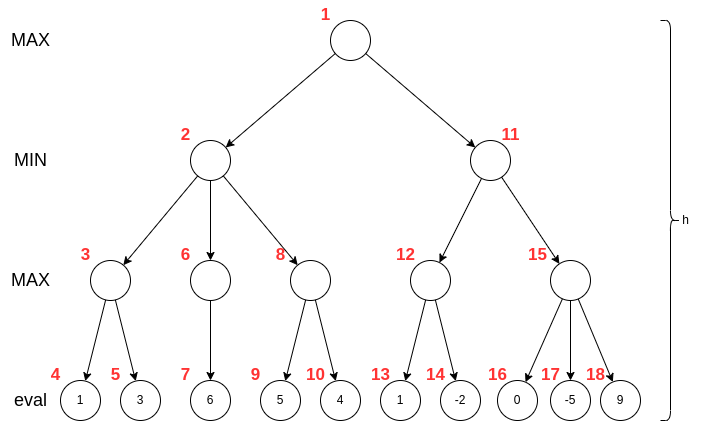
\includegraphics[scale=.6]{graphics/minimax_kolejnosc.png}
    \caption{Kolejność rozpatrywania stanów przez Minimax dla h = 3}
    \label{fig:kolejnosc}
\end{figure}

\begin{figure}
    \centering
    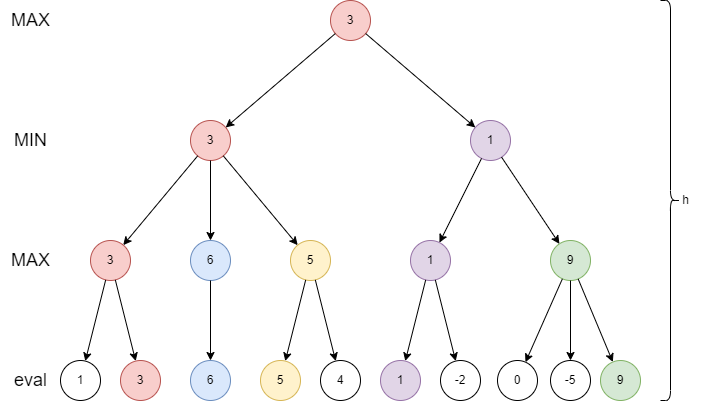
\includegraphics[scale=.6]{graphics/minimax_przebieg.png}
    \caption{Wynik przebiegu Minimaxa dla przykładu dla h = 3}
    \label{fig:minimax}
\end{figure}

\subsection{Alpha-Beta-pruning}

Patrząc jeszcze raz na~rys.~\ref{fig:kolejnosc} i~rys.~\ref{fig:minimax} można zauważyć, że posiadając wiedzę o wartościach ocen odwiedzonych już stanów, nie ma potrzeby rozpatrywania niektórych następujących stanów. Na przykład w stanie numer 8, wiedząc że jego pierwsze dziecko otrzymało ocenę 5, można być pewnym że MAX dla tego stanu wybierze stan o wartości co najmniej 5, co sprawi że gracz MIN nad nim będzie miał do rozpatrzenia stany o~wartościach dokładnie 3, dokładnie 6, co najmniej 5. Jako że gracz ten minimalizuje, wybierze stan o~wartości 3. Wynika stąd, że sprawdzenie drugiego dziecka stanu numer 8 byłoby niepotrzebne, ponieważ nie wpłynęłoby na ostateczny wynik. Można też obciąć całe poddrzewo z korzeniem w stanie numer 15 - wybór gracza MIN będzie miał ocenę ograniczoną z góry przez 1, więc gracz MAX na pewno nie poprawi wyniku idąc tą ścieżką, wiedząc że ma obok stan o lepszej ocenie. Zaoszczędzono w ten sposób zasoby na przejrzenie 5 stanów, w tym jednego poddrzewa.~(Rys.~\ref{fig:alpha_beta})

Taką optymalizację nazywa się cięciami alfa-beta~\cite{Modern}. Są to rezygnacje z rozpatrywania innych podgałęzi ze względu na brak możliwości poprawienia wyniku. Zoptymalizowany w ten sposób Minimax w~trakcie działania operuje dwiema wartościami: $\alpha$ i $\beta$. $\alpha$ reprezentuje najwyższą ocenę znaną w poddrzewie, $\beta$~natomiast - najniższą. Wartości $\alpha$ i $\beta$ aktualizowane są w poddrzewach przez odpowiednio gracza MAX i gracza MIN. W momencie gdy $\beta \leq \alpha$, rekurencyjne wywołanie Minimaxa w poddrzewie zostaje zakończone i zwracana jest najlepsza (zdaniem gracza) wartość.

\begin{figure}
    \centering
    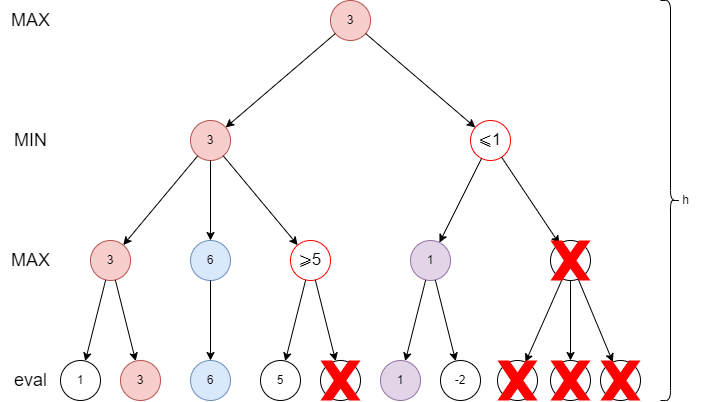
\includegraphics[scale=.6]{graphics/minimax_alfa-beta.png}
    \caption{Zastosowanie cięć alfa-beta na przykładzie}
    \label{fig:alpha_beta}
\end{figure}

Wadą cięć alfa-beta jest ich zależność od kolejności rozpatrywania węzłów - gdyby algorytm w przykładzie~\ref{fig:minimax} wpierw przeszedł przez poddrzewo numer 15, musiałby przejrzeć jeszcze poddrzewo numer 12, bo nie byłby pewny co do możliwości poprawienia wyniku dla rodzica. Mankament ten sprawia, że stosunku liczby optymalizowanych stanów do całego poddrzewa nie da się jednoznacznie określić.

\section{Funkcja oceny heurystycznej}

Ze względu na ogromny rozmiar przestrzeni stanów w warcabach, obecne komputery nie potrafią przeszukać jej całości w ,,rozsądnym'' czasie. Jeśli jednym z celów budowania sztucznej inteligencji są w~miarę szybkie decyzje prowadzące do zwycięstwa w grze, należy skrócić przeszukiwanie przestrzeni stanów i w jakiś sposób obejść się z niedoskonałą informacją posiadaną przez komputer. Ocena danego stanu na planszy ma wspomóc taki komputer w wyrobieniu ,,intuicji'' poprzez analizę sytuacji na planszy.

\FloatBarrier

Podejście w pracy do funkcji oceny heurystycznej polega na rozpatrzeniu wielu parametrów na planszy (np. liczba pionów, liczba damek przeciwnika, liczba ruchów), przemnożeniu wartości tych parametrów przez ustalone z góry wagi, a na koniec zsumowaniu powstałych iloczynów. Suma tych iloczynów to wartość funkcji oceny, którą przypisuje się pod dany stan gry.

Wartość funkcji oceny heurystycznej można określić następującym wzorem:
{\centering
$\sum_{i=1}^{n}(param_i * weight_i)$
}.

Funkcja oceny heurystycznej zależy oczywiście od podjętej strategii oraz od podejścia do problemu. Opisana wyżej funkcja ma parę zalet, na których opiera się praca. Po pierwsze, wyznaczenie oceny z~wyliczonymi już wartościami parametrów odbywa się szybko, bo w czasie liniowym (nie uwzględnia to czasu potrzebnego do rozpatrzenia tychże parametrów). Po drugie, listowanie parametrów w ten sposób pozwala na przeprowadzenie eksperymentów i wyciągnięcie wniosków na temat teorii gry w warcaby, o~czym w~poniższym podrozdziale.

\subsection{Wykorzystywane parametry}

\FloatBarrier

% \label{params}

{
% \small
\begin{center}
\begin{table}
\centering
{\footnotesize
\begin{tabular}{|c | c || c | c|}
 \hline
 Nr & Parametr & Nr & Parametr \\ %[0.5ex] 
 \hline\hline
 1 & Liczba sojuszniczych pionów & 31 & Liczba przeciwnych pionów w środkowych rzędach \\ 
 \hline
 2 & Liczba sojuszniczych damek & 32 & Liczba przeciwnych damek w środkowych wierszach \\
 \hline
 3 & Liczba przeciwnych pionów & 33 & Liczba sojuszniczych pionów w górnych rzędach \\
 \hline
 4 & Liczba przeciwnych damek & 34 & Liczba sojuszniczych damek w górnych rzędach \\
 \hline
 5 & Liczba sojuszniczych pionów przy ścianie & 35 & Liczba przeciwnych pionów w górnych rzędach \\
 \hline
 6 & Liczba sojuszniczych damek przy ścianie & 36 & Liczba przeciwnych damek w górnych rzędach \\ 
 \hline
 7 & Liczba przeciwnych pionów przy ścianie & 37 & Liczba samotnych sojuszniczych pionów \\
 \hline
 8 & Liczba przeciwnych damek przy ścianie & 38 & Liczba samotnych sojuszniczych damek \\
 \hline
 9 & Liczba ruchomych pionów gracza & 39 & Liczba samotnych przeciwnych pionów \\
 \hline
 10 & Liczba ruchomych damek gracza & 40 & Liczba samotnych przeciwnych damek \\
 \hline
 11 & Liczba ruchomych pionów przeciwnika & 41 & Czy pion gracza jest w kącie \\ 
 \hline
 12 & Liczba ruchomych damek przeciwnika & 42 & Czy damka gracza jest w kącie \\
 \hline
 13 & Liczba możliwych ruchów gracza & 43 & Czy gracz zajmuje dwa kąty \\
 \hline
 14 & Liczba możliwych ruchów przeciwnika & 44 & Czy pion przeciwnika jest w kącie \\
 \hline
 15 & Istnienie bijącego ruchu gracza & 45 & Czy damka przeciwnika jest w kącie \\
 \hline
 16 & Liczba bijących ruchów gracza & 46 & Czy przeciwnik zajmuje dwa kąty \\ 
 \hline
 17 & Rozmiar najdłuższego bijącego ruchu gracza & 47 & Obecność \textit{Triangle pattern} u gracza \\
 \hline
 18 & Istnienie bijącego ruchu przeciwnika & 48 & Obecność \textit{Oreo pattern} u gracza \\
 \hline
 19 & Liczba bijących ruchów przeciwnika & 49 & Obecność \textit{Bridge pattern} u gracza \\
 \hline
 20 & Rozmiar najdłuższego bijącego ruchu przeciwnika & 50 & Obecność \textit{Dog pattern} u gracza \\
 \hline
 21 & Suma dystansów pionów gracza do rzędu awansu & 51 & Obecność \textit{Triangle pattern} u przeciwnika \\ 
 \hline
 22 & Suma dystansów pionów przeciwnika do rzędu awansu & 52 & Obecność \textit{Oreo pattern} u przeciwnika \\
 \hline
 23 & Liczba niezajętych pól w rzędzie awansu gracza & 53 & Obecność \textit{Bridge pattern} u przeciwnika \\
 \hline
 24 & Liczba niezajętych pól w rzędzie awansu przeciwnika & 54 & Obecność \textit{Dog pattern} u przeciwnika \\
 \hline
 25 & Liczba sojuszniczych pionów w dolnych rzędach & 55 & Liczba blokujących sojuszniczych figur \\
 \hline
 26 & Liczba sojuszniczych damek w dolnych rzędach & 56 & Liczba linii bloku gracza \\ 
 \hline
 27 & Liczba przeciwnych pionów w dolnych rzędach & 57 & Wielkość najdłuższej linii bloku gracza \\
 \hline
 28 & Liczba przeciwnych damek w dolnych rzędach & 58 & Liczba blokujących przeciwnych figur \\
 \hline
 29 & Liczba sojuszniczych pionów w środkowych rzędach & 59 & Liczba linii bloku przeciwnika \\
 \hline
 30 & Liczba sojuszniczych damek w środkowych rzędach & 60 & Wielkość najdłuższej linii bloku przeciwnika \\
 \hline
\end{tabular}
}
\caption[ Parametry funkcji oceny heurystycznej ]{Wszystkie parametry rozpatrywane w pracy. Część parametrów została zaczerpnięta z \cite{EvoCheckers}.}
\label{tab:params}
\end{table}
\end{center}
}

\label{params}

{
% \small
\begin{center}
\begin{table}
\centering
{\footnotesize
\begin{tabular}{|c | c || c | c|}
 \hline
 Nr & Parametr & Nr & Parametr \\ %[0.5ex] 
 \hline\hline
 1 & Liczba sojuszniczych pionów & 31 & Liczba przeciwnych pionów w środkowych rzędach \\ 
 \hline
 2 & Liczba sojuszniczych damek & 32 & Liczba przeciwnych damek w środkowych wierszach \\
 \hline
 3 & Liczba przeciwnych pionów & 33 & Liczba sojuszniczych pionów w górnych rzędach \\
 \hline
 4 & Liczba przeciwnych damek & 34 & Liczba sojuszniczych damek w górnych rzędach \\
 \hline
 5 & Liczba sojuszniczych pionów przy ścianie & 35 & Liczba przeciwnych pionów w górnych rzędach \\
 \hline
 6 & Liczba sojuszniczych damek przy ścianie & 36 & Liczba przeciwnych damek w górnych rzędach \\ 
 \hline
 7 & Liczba przeciwnych pionów przy ścianie & 37 & Liczba samotnych sojuszniczych pionów \\
 \hline
 8 & Liczba przeciwnych damek przy ścianie & 38 & Liczba samotnych sojuszniczych damek \\
 \hline
 9 & Liczba ruchomych pionów gracza & 39 & Liczba samotnych przeciwnych pionów \\
 \hline
 10 & Liczba ruchomych damek gracza & 40 & Liczba samotnych przeciwnych damek \\
 \hline
 11 & Liczba ruchomych pionów przeciwnika & 41 & Czy pion gracza jest w kącie \\ 
 \hline
 12 & Liczba ruchomych damek przeciwnika & 42 & Czy damka gracza jest w kącie \\
 \hline
 13 & Liczba możliwych ruchów gracza & 43 & Czy gracz zajmuje dwa kąty \\
 \hline
 14 & Liczba możliwych ruchów przeciwnika & 44 & Czy pion przeciwnika jest w kącie \\
 \hline
 15 & Istnienie bijącego ruchu gracza & 45 & Czy damka przeciwnika jest w kącie \\
 \hline
 16 & Liczba bijących ruchów gracza & 46 & Czy przeciwnik zajmuje dwa kąty \\ 
 \hline
 17 & Rozmiar najdłuższego bijącego ruchu gracza & 47 & Obecność \textit{Triangle pattern} u gracza \\
 \hline
 18 & Istnienie bijącego ruchu przeciwnika & 48 & Obecność \textit{Oreo pattern} u gracza \\
 \hline
 19 & Liczba bijących ruchów przeciwnika & 49 & Obecność \textit{Bridge pattern} u gracza \\
 \hline
 20 & Rozmiar najdłuższego bijącego ruchu przeciwnika & 50 & Obecność \textit{Dog pattern} u gracza \\
 \hline
 21 & Suma dystansów pionów gracza do rzędu awansu & 51 & Obecność \textit{Triangle pattern} u przeciwnika \\ 
 \hline
 22 & Suma dystansów pionów przeciwnika do rzędu awansu & 52 & Obecność \textit{Oreo pattern} u przeciwnika \\
 \hline
 23 & Liczba niezajętych pól w rzędzie awansu gracza & 53 & Obecność \textit{Bridge pattern} u przeciwnika \\
 \hline
 24 & Liczba niezajętych pól w rzędzie awansu przeciwnika & 54 & Obecność \textit{Dog pattern} u przeciwnika \\
 \hline
 25 & Liczba sojuszniczych pionów w dolnych rzędach & 55 & Liczba blokujących sojuszniczych figur \\
 \hline
 26 & Liczba sojuszniczych damek w dolnych rzędach & 56 & Liczba linii bloku gracza \\ 
 \hline
 27 & Liczba przeciwnych pionów w dolnych rzędach & 57 & Wielkość najdłuższej linii bloku gracza \\
 \hline
 28 & Liczba przeciwnych damek w dolnych rzędach & 58 & Liczba blokujących przeciwnych figur \\
 \hline
 29 & Liczba sojuszniczych pionów w środkowych rzędach & 59 & Liczba linii bloku przeciwnika \\
 \hline
 30 & Liczba sojuszniczych damek w środkowych rzędach & 60 & Wielkość najdłuższej linii bloku przeciwnika \\
 \hline
\end{tabular}
}
\caption[ Parametry funkcji oceny heurystycznej ]{Wszystkie parametry rozpatrywane w pracy. Część parametrów została zaczerpnięta z \cite{EvoCheckers}.}
\label{tab:params}
\end{table}
\end{center}
}


W tabeli~\ref{tab:params} przedstawione są wszystkie wykorzystywane w pracy parametry. Są to liczby i flagi wyciągane z danego stanu rozgrywki i wykorzystywane do obliczenia wartości funkcji oceny heurystycznej dla tego stanu. Duża część tych parametrów to symetryczne odbicia innych parametrów względem figury (pion/damka) lub względem gracza (MAX/MIN). Poniżej znajduje się krótkie objaśnienie niektórych parametrów.

\begin{itemize}
    \item \textbf{[9-12] Ruchome figury} to figury, które są w stanie wykonać co najmniej jeden ruch (w tym bicie).
    \item \textbf{[13-14] Możliwe ruchy graczy} są obliczane nawet jeśli w rozpatrywanym stanie tura nie należy do tego gracza.
    \item \textbf{[21-24] Rzędem awansu gracza} nazywamy rząd, w którym pion gracza awansuje do damki. \textbf{dystansem piona do rzędu} nazywamy liczbę pól w linii prostej od piona do rzędu.
    \item \textbf{[25-36] Dolne, środkowe i górne rzędy} gracza~/~przeciwnika rozważa się z perspektywy gracza~/~przeciwnika. \textbf{Dolne rzędy} gracza oznaczają dwa rzędy najbliżej gracza, \textbf{górne rzędy} gracza to trzy rzędy najbliższe jego przeciwnika, natomiast \textbf{środkowymi rzędami} nazywa się dwa rzędy w centrum planszy.
    \item \textbf{[37-40] Samotne figury} to takie, które nie mają w najbliższym sąsiedztwie żadnej figury.
    \item \textbf{[15, 18, 41-54]} Niektóre parametry są \textbf{parametrami binarnymi} i jako wartość przyjmują 0 lub~1.
    \item \textbf{[47-54] Każdy wspomniany ,,pattern''} jest objaśniony na ilustracjach~\ref{fig:patterns}.
    \item \textbf{[55-60] Blokujące figury} w tych parametrach to takie, które znajdują się za sojuszniczą figurą i~tym samym blokują możliwość zbicia chronionej figury. \textbf{Linia bloku} składa się z co najmniej dwóch figur danego gracza ustawionych obok siebie na przekątnej.
\end{itemize}

\begin{figure*}
    \centering
    \begin{subfigure}[b]{0.475\textwidth}
        \centering
        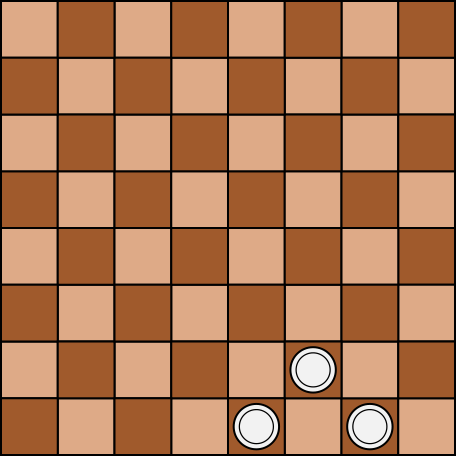
\includegraphics[scale=.6]{graphics/warcaby_patternTriangle.png}
        \caption[Network2]%
        {{Triangle pattern}}    
        \label{fig:pattern_triangle}
    \end{subfigure}
    \hfill
    \begin{subfigure}[b]{0.475\textwidth}  
        \centering 
        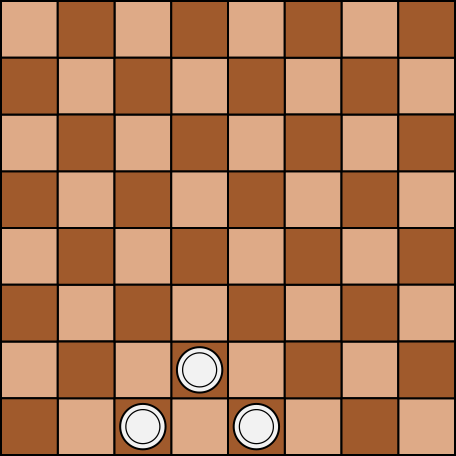
\includegraphics[scale=.6]{graphics/warcaby_patternOreo.png}
        \caption[]%
        {{Oreo pattern}}    
        \label{fig:pattern_oreo}
    \end{subfigure}
    \vskip\baselineskip
    \begin{subfigure}[b]{0.475\textwidth}   
        \centering 
        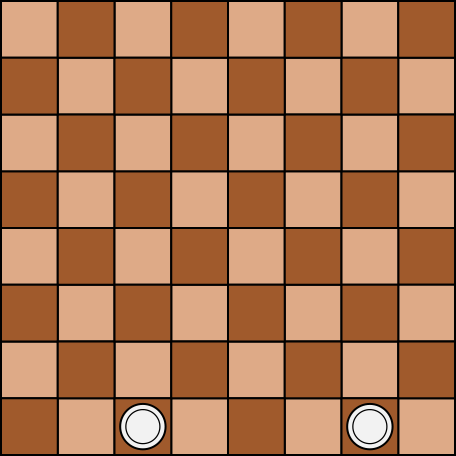
\includegraphics[scale=.6]{graphics/warcaby_patternBridge.png}
        \caption[]%
        {{Bridge pattern}}    
        \label{fig:pattern_bridge}
    \end{subfigure}
    \hfill
    \begin{subfigure}[b]{0.475\textwidth}   
        \centering 
        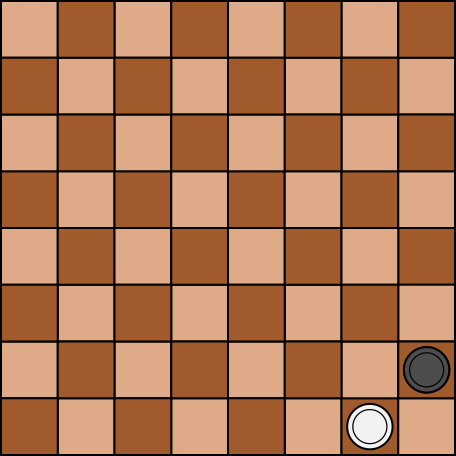
\includegraphics[scale=.6]{graphics/warcaby_patternDog.png}
        \caption[]%
        {{Dog pattern}}    
        \label{fig:pattern_dog}
    \end{subfigure}
    \caption{Wzory na planszy względem gracza białego, wykorzystywane do niektórych parametrów} 
    \label{fig:patterns}
\end{figure*}

\FloatBarrier

\section{Algorytm genetyczny}
\label{podrozdzial2-3}

Jednym z najważniejszych celów pracy jest znalezienie odpowiedniej strategii gry w warcaby w postaci dobrej funkcji oceny heurystycznej, co w tym przypadku sprowadza się do wyznaczenia jak najlepszego zestawu wartości wag, dalej zwanego ciągiem wag. Naiwnym podejściem do tego problemu byłoby przypisanie priorytetów każdego parametru stanu planszy przez człowieka bądź zespół ludzi. Może się jednak okazać, że pewne parametry nie będą tak wartościowe dla zwycięstwa jak podpowiedziałaby ludzka intuicja. Ponadto, zakładając że nie istnieje obiektywne spojrzenie na jakość danej strategii, należałoby przeprowadzić ogromną liczbę testów gry z człowiekiem w celu sprawdzenia poprawności wyznaczonych wag (tj. czy podane wartości ciągu wag są wystarczające by algorytm uznać za kompetytywnego gracza). Z pomocą tutaj przychodzi zastosowanie algorytmu genetycznego.

Algorytm genetyczny jest przedstawicielem klasy algorytmów metaheurystycznych. Konkretniej jest to odmiana algorytmu ewolucyjnego, który z kolei jest pochodną algorytmu populacyjnego. Metaheurystyka genetyczna symuluje zjawisko doboru naturalnego w przyrodzie, operując kolejnymi pokoleniami populacji osobników reprezentującymi potencjalne rozwiązania danego problemu, starając się odnaleźć rozwiązanie suboptymalne.

Najprostszy zarys algorytmu genetycznego można zobrazować w następujący sposób. W początkowej populacji losowo utworzonych osobników (rozwiązań), nazwaną pierwszym pokoleniem, dochodzi do selekcji, mającej na celu wyznaczenie populacji rodziców. W populacji rodziców dochodzi do wzajemnego krzyżowania i tworzenia się populacji dzieci, które dziedziczą po swoich rodzicach informacje genetyczne (tj. elementy rozwiązania). Wśród dzieci może z pewnym prawdopodobieństwem dojść do mutacji, która losowo zmienia jeden z elementów genotypu u osobnika. Dzieci, wraz z niektórymi rodzicami lub nowymi, losowymi osobnikami (zależnie od wersji), określa się nowym pokoleniem. W populacji nowego pokolenia powtarza się proces selekcji, krzyżowania i mutacji, aż do osiągnięcia z góry ustalonego warunku stopu (np. limitu czasowego).~(Rys.~\ref{fig:alggen})

\begin{figure}
    \centering
    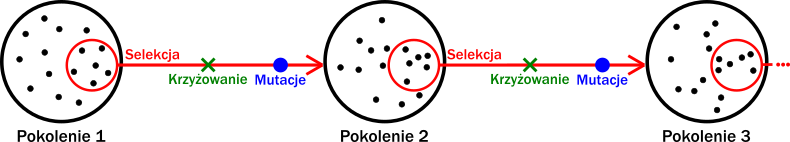
\includegraphics[scale=.7]{graphics/genetyk_algorytm.png}
    \caption{Ogólny przebieg algorytmu genetycznego}
    \label{fig:alggen}
\end{figure}

Biorąc pod uwagę fakt, że to od rodziców zależy jakość każdej populacji, szczególny nacisk należy położyć na fazę selekcji. Niezbyt intuicyjną, a ważną taktyką jest też wprowadzanie w pewne miejsca przebiegu algorytmu elementów losowości, aby w populacji nie dochodziło do tak zwanego zjawiska stagnacji (sytuacji, w której zbyt wiele osobników w populacji jest do siebie bardzo podobnych) oraz aby algorytm był w stanie znajdować inne, być może lepsze, rozwiązania.

\subsection{Populacja i osobniki}

Osobnikiem populacji będzie ciąg wag funkcji oceny heurystycznej, reprezentowany jako tablica liczb całkowitych. Wagi będą mogły przyjmować zarówno dodatnie, jak i ujemne wartości.~(Rys.~\ref{fig:osobnik})

\begin{figure}
    \centering
    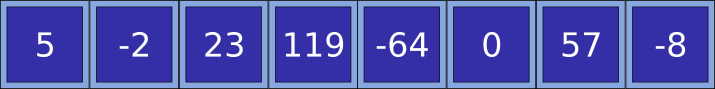
\includegraphics[scale=.6]{graphics/genetyk_osobnik.png}
    \caption{Uproszczony model osobnika (ciągu wag)}
    \label{fig:osobnik}
\end{figure}

\subsection{Selekcja i ewaluacja}

W wielu problemach, do których stosuje się algorytmy genetyczne, funkcja ewaluacji osobnika jest podana w treści problemu bądź łatwa do wyznaczenia. Tak jednak nie jest z problemem znalezienia najlepiej grającej sztucznej inteligencji. Dlatego też zastosowane zostało podejście lokalne, czyli zwracające uwagę na umiejętności osobników w danej populacji. W procesie selekcji każdy ciąg wag gra z każdym innym ciągiem wag w podwójnym pojedynku (białe/czarne i czarne/białe). Im więcej gier wygra dany ciąg wag, tym wyższe prawdopodobieństwo, że zostanie on wylosowany do populacji rodziców.

\subsection{Krzyżowanie i mutacja}

W pracy zaimplementowano dobieranie rodziców w pary w których się wzajemnie krzyżują, produkując dwójkę dzieci. Aby zachować potencjalnie dobre informacje genetyczne, dzieli się ciągi wag rodziców w~tym samym losowo wyznaczonym miejscu i zamienia się ze sobą części. Dzięki temu każde z dwójki dzieci przechowuje cechy po każdym swoim rodzicu.~(Rys.~\ref{fig:krzyzowanie})

\begin{figure}
    \centering
    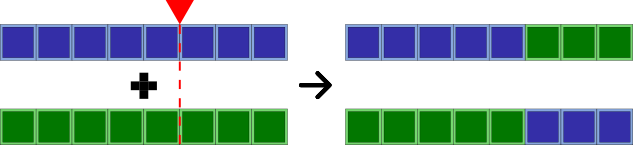
\includegraphics[scale=.6]{graphics/genetyk_krzyzowanie2.png}
    \caption{Model krzyżowania dwóch osobników w implementacji}
    \label{fig:krzyzowanie}
\end{figure}

Mutacja u nowo narodzonych osobników następuje z pewnym prawdopodobieństwem i wpływa na maksymalnie jedną wartość w~ciągu wag. Mutowana waga zostaje zastąpiona losową wartością z odpowiedniego przedziału.


